\section{D meson selection}
\Dzero, \Dplus, \Dstar and \Dsubs mesons and their anti-particles are reconstructed in the central rapidity region by exploiting their charged hadronic decay channels: \Dzero $\rightarrow$ K$^{-}\pi^{+}$ (with branching ratio B.R. = 3.89 $\pm$ 0.05$\%$ and mean proper decay length $c\tau$ = 123 $\mu$m), \Dplus $\rightarrow$ K$^{-}\pi^{+}\pi^{+}$ (with B.R. = 8.98 $\pm$ 0.28$\%$ and \mbox{$c\tau$ = 312 $\mu$m}), \Dstar $\rightarrow$ \Dzero$\pi^{+}$ (with B.R. = 67.7 $\pm$ 0.5$\%$) and \Dsubs $\rightarrow$ K$^{-}$K$^{+}\pi^{+}$ (with \mbox{B.R. = 2.27 $\pm$ 0.08$\%$}).
The selection of \Dzero and \Dplus candidates is based on the reconstruction of the displaced secondary vertex topologies, with a typical separation of $\sim$ 100--300 $\mu$m from the interaction point. The \Dstar decay proceeds via strong interaction, thus making impossible the secondary vertex reconstruction. In this case the selection is applied to the decay topology of the daughter \Dzero. \Dsubs mesons are reconstructed via the decay channel \Dsubs $\rightarrow$ K$^{-}$K$^{+}\pi^{+}$, exploiting the resonant decay channel $\phi \rightarrow$ K$^{-}$K$^{+}$ (with \mbox{B.R. = 2.28 $\pm$ 0.12$\%$} and $c\tau \approx$ 150 $\mu$m).
The D mesons raw yields are extracted from the invariant mass distributions obtained from the analysis of fully reconstructed decay topologies displaced with respect to the primary vertex.
\subsection{Single track selections}
\label{sec:single_track}
Secondary vertices of \Dzero and \Dplus meson candidates were constructed using tracks having $|\eta| <$ 0.8, \pt $>$ 0.5 GeV/$c$ and satisfying the kITSrefit and kTPCrefit conditions. Moreover, for all the tracks, a minimum number of 70 crossed rows in the TPC together with a crossed rows over findable clusters ratio of 0.8 was required. A cut on the transverse impact parameter $d_0$ was applied for tracks with \pt $<$ 2 GeV/$c$, requiring $d_0 >$ 50 $\mu$m. These selections were meant to limit the CPU time needed to perform the track combinatorics when creating the AODs with the D meson candidates. Furthermore, all tracks, including the \Dstar soft pion, were selected requiring at least 70 (out of a maximum of 159) associated space points and $\chi^2$/$ndf <$ 2 in the TPC, and at least one associated hit in either of the two SPD layers.

\subsection{Topological and kinematic selections}
The signal extraction is based on topological selections of displaced secondary vertices from D-meson candidates. For a detailed explanation of the procedure refer to \cite{Adam:2015sza}. The topological and kinematic cuts used to select the D-meson signal in 0--10$\%$ and 30--50$\%$ collisions from 2018 data sample \pbpb collisions are reported in Table \ref{tab:dzero}, \ref{tab:dplus}, \ref{tab:dstar}, \ref{tab:dsubs} for the analyses in 0--10$\%$ and in Table \ref{tab:dzero2}, \ref{tab:dplus2}, \ref{tab:dstar2}, \ref{tab:dsubs2} for the analyses in 30--50$\%$.

The same topological and kinematic variables used for the analyses with the 2015 \pbpb data sample are reported. In particular, we recall the introduction of a topological variable introduced in \cite{Bruna:2016mgn} : the normalized impact parameter (IP) resolution. It is defined as the difference between the expected impact parameter value $d^{exp}_{0,T,\phi} \approx L_{xy} \cdot sin(\theta_{xy})$, where $L_{xy}$ is the decay length on $xy$ plane and $\theta_{xy}$ is the angle between the reconstructed D meson and the charged particle on $xy$ plane, and the reconstructed one $d^{reco}_{0,T,\phi}$. This difference is then normalized by the square root of their respective uncertainties summed in quadrature. A selection based on this variable can reduce the feed-down D-meson efficiency while keeping higher that of prompt D mesons. The projections of the variables in the $xy$ plane are instead justified by the improving of the impact parameter resolution with respect to $z$-direction. More details on this variable can be found in \cite{Bruna:2016mgn}.

In addition, \Dsubs candidates were selected by requiring that one of the two pairs of oppositely-charged tracks had an invariant mass compatible with the PDG world average for the $\phi$ mass (1.019 GeV/$c^2$). 
%In order to further suppress the combinatorial background, the angles $\theta^{*}(\pi)$ and $\theta^{'}$(K) were exploited. 
%The first one is the angle between the pion in the KK$\pi$ rest frame and the KK$\pi$ flight line, which is defined by the positions of the primary and secondary vertices in the laboratory frame, and the second one is the angle between one of the two kaons and the pions in the KK rest frame.
In order to further suppress the combinatorial background, the angle $\theta^{'}$(K) was exploited. This is the angle between one of the two kaons and the pions in the KK rest frame.



\begin{table}[h!]
  \begin{center}
    \caption{Topological and kinematic selections applied for the \Dstar analysis in 30--50$\%$ centrality class.}
    \label{tab:dstar2}
    \resizebox{\linewidth}{!}{\begin{tabular}{|c|c|c|c|c|c|c|c|c|c|c|c|c|}
    \hline
      \pt (GeV/$c$) variable & [2,3] & [3,4] & [4,5] & [5,6] & [6,7] & [7,8] & [8,10] & [10,12] & [12,16] & [16,24] & [24,36] \\
      \hline
      \hline
      $\Delta M_{D^0}$ (Gev)  & 0.024 & 0.032 & 0.032 & 0.04 & 0.043 & 0.045 & 0.055 & 0.06 & 0.074 & 0.74 & 0.094\\
      \hline
      DCA (cm) & 0.023 & 0.022 & 0.022 & 0.021 & 0.021 & 0.021 & 0.021 & 0.021 & 0.021 & 0.02 &  0.02 \\
      \hline
      $Cos(\theta^*)$ & 0.8 & 0.8 & 0.8 & 1.0 & 1.0 & 1.0 & 1.0 & 1.0 & 1.0 & 1.0 & 1.0  \\
      \hline
      \pt($K$) (GeV/$c$) & 1.0 &  1.0 & 1.0 & 1.0 & 1.0 & 0.9 & 0.9 & 0.7 &  & 0.5 & 0.5 \\
      \hline
      \pt($\pi$) (GeV/$c$) & 1.0 & 1.0 & 1.0 & 1.0 & 1.0 & 1.0 & 1.0 & 1.0 & 0.5 & 0.5 & 0.5 \\
      \hline
      $d_{0,K}$ (cm) & 0.1 & 0.1 & 0.1  & 0.1 & 0.1 & 0.12 & 0.12 & 0.15 & 0.15 & 0.15 & 0.2\\
	  \hline
	  $d_{0,\pi}$ (cm) & 0.1 & 0.1 & 0.1 & 0.1 & 0.1 & 0.12 & 0.12 & 0.15 &0.15  &0.15  &0.2 \\
	  \hline
	  $d_{0,K} \times d_{0,\pi}$ (10$^{-3}$) (cm$^2$) & -0.00032   &-0.0003  &  -0.0003& -0.00023 & -0.0001 &-0.0001  & -7.5 $\times 10^{-5}$ &-7.5 $\times 10^{-5}$  & -5 $\times 10^{-5}$ & -5 $\times 10^{-5}$ &0.0004 \\
	  \hline
	  $Cos(\theta_{point})$ & 0.93 & 0.93 & 0.93  & 0.93 & 0.93 & 0.93 & 0.93 & 0.93 & 0.93 & 0.85 & 0.85  \\
	  \hline
	  $Cos(\theta_{point})XY$ & 0.998 & 0.998 & 0.998 & 0.998 & 0.998 & 0.998 & 0.998 & 0.99 & 0.99 & 0.9 &0.9 \\
	  \hline
	  $L_{XY}$ & 7 & 6.7 & 6.5 & 6.5 & 6.4 & 6.4 & 4.7 & 4.7 & 3.7 & 1 &  0 \\
	  \hline
    \end{tabular}
    }
  \end{center}
\end{table}



\subsection{Particle identification}
\label{sec:pid_sel}
The identification of the charged kaons and pions in the TPC and TOF detectors provide an additional information for the background rejection in the low momentum region. In order to assign K and/or $\pi$ masses to the decay tracks, cuts are applied to the difference in the expected and measured signals, which are the specific energy deposited (d$E$/d$x$) in the TPC and the time-of-flight for the TOF. A 3$\sigma$ compatibility was required to \Dzero, \Dstar and \Dplus candidate's daughters. When tracks were without TOF signal, only the TPC particle identification was used. Tracks with contradicting particle identification were considered to be non-identified and retained for further analysis. 
For the \Dsubs, cuts were applied to the difference between the measured signals and those expected for a pion or a kaon. For \pt $<$ 8 GeV/$c$, where the signal over background is small, a track was considered compatible with the kaon or pion hypothesis if both its d$E$/d$x$ and time-of-flight were within 3$\sigma$ from the expected values. Tracks without a TOF signal (mostly at low momentum) were identified using only the TPC information and requiring a 2$\sigma$ compatibility with the expected specific energy loss. Triplets of selected tracks were required to have two tracks compatible with the kaon hypothesis and one with the pion hypothesis. In addition, since the decay particle with opposite charge sign has to be a kaon, a triplet was rejected if the opposite-sign track was not compatible with the kaon hypothesis. This particle identification strategy, applied at low momentum, preserves about 85$\%$ of the \Dsubs signal.

\subsection{Signal extraction}
\label{sec:sign_extr}
The \Dzero and \Dsubs raw yields were extracted by performing a fit to the invariant mass distribution with a function composed of a Gaussian for the signal and an exponential to interpolate the background shape. In particular, for \Dzero the exponential is used for \pt $>$ 3 GeV/$c$, while a pol3 and pol2 where used for 1-2 GeV/$c$ and 2-3 GeV/$c$ bins, respectively. In case of \Dplus, signals are fitted with Gaussian and background is fitted with Polynomial2 which describes the shape of the background reasonably well. In the case of the \Dstar the fit was performed to the mass difference $\Delta M$ = $M$(K$\pi\pi$) - $M$(K$\pi$) distributions and the term describing the background shape is an exponential convoluted with a power law according to the equation:
\begin{equation}
	f_{bkg} = a\sqrt{\Delta M - m_{\pi}}\cdot e^{b(\Delta M - m_{\pi})}
\end{equation}
where $m_{\pi}$ is the pion mass and $a$ and $b$ are free parameters.

For all the four mesons the signal was extracted in the 0--10$\%$ centrality class in several transverse momentum regions: 
\begin{itemize}
	%\item for \Dzero in the range 1-50 GeV/$c$;
	\item for \Dstar in the range 1-50 GeV/$c$;
	%\item for \Dplus in the range 2-50 GeV/$c$;
	%\item for \Dsubs in the range 3-36 GeV/$c$;
\end{itemize} 
The invariant-mass distributions obtained in 0--10$\%$ centrality class are reported in Fig.~\ref{fig:DzeroInvMassFits_cent_lowpt,fig:DzeroInvMassFits_cent_highpt} for \Dzero, in Fig.~\ref{fig:Dstar_InvMass} for \Dstar, in Fig.~\ref{fig:Dplus_InvMass}  for \Dplus and in Fig.~\ref{fig:DsubsInvMassFits_cent} for \Dsubs. For the \Dzero in the \pt bin 36-50 GeV/$c$, the fit is performed by fixing the mean  and the width to the values obtained from the MC, once it was checked that the MC properly reproduce the mean and width of the \Dzero Gaussian peak.



% Dstar 0-10% InvMass plot
\begin{figure}[tb]
\begin{center}
 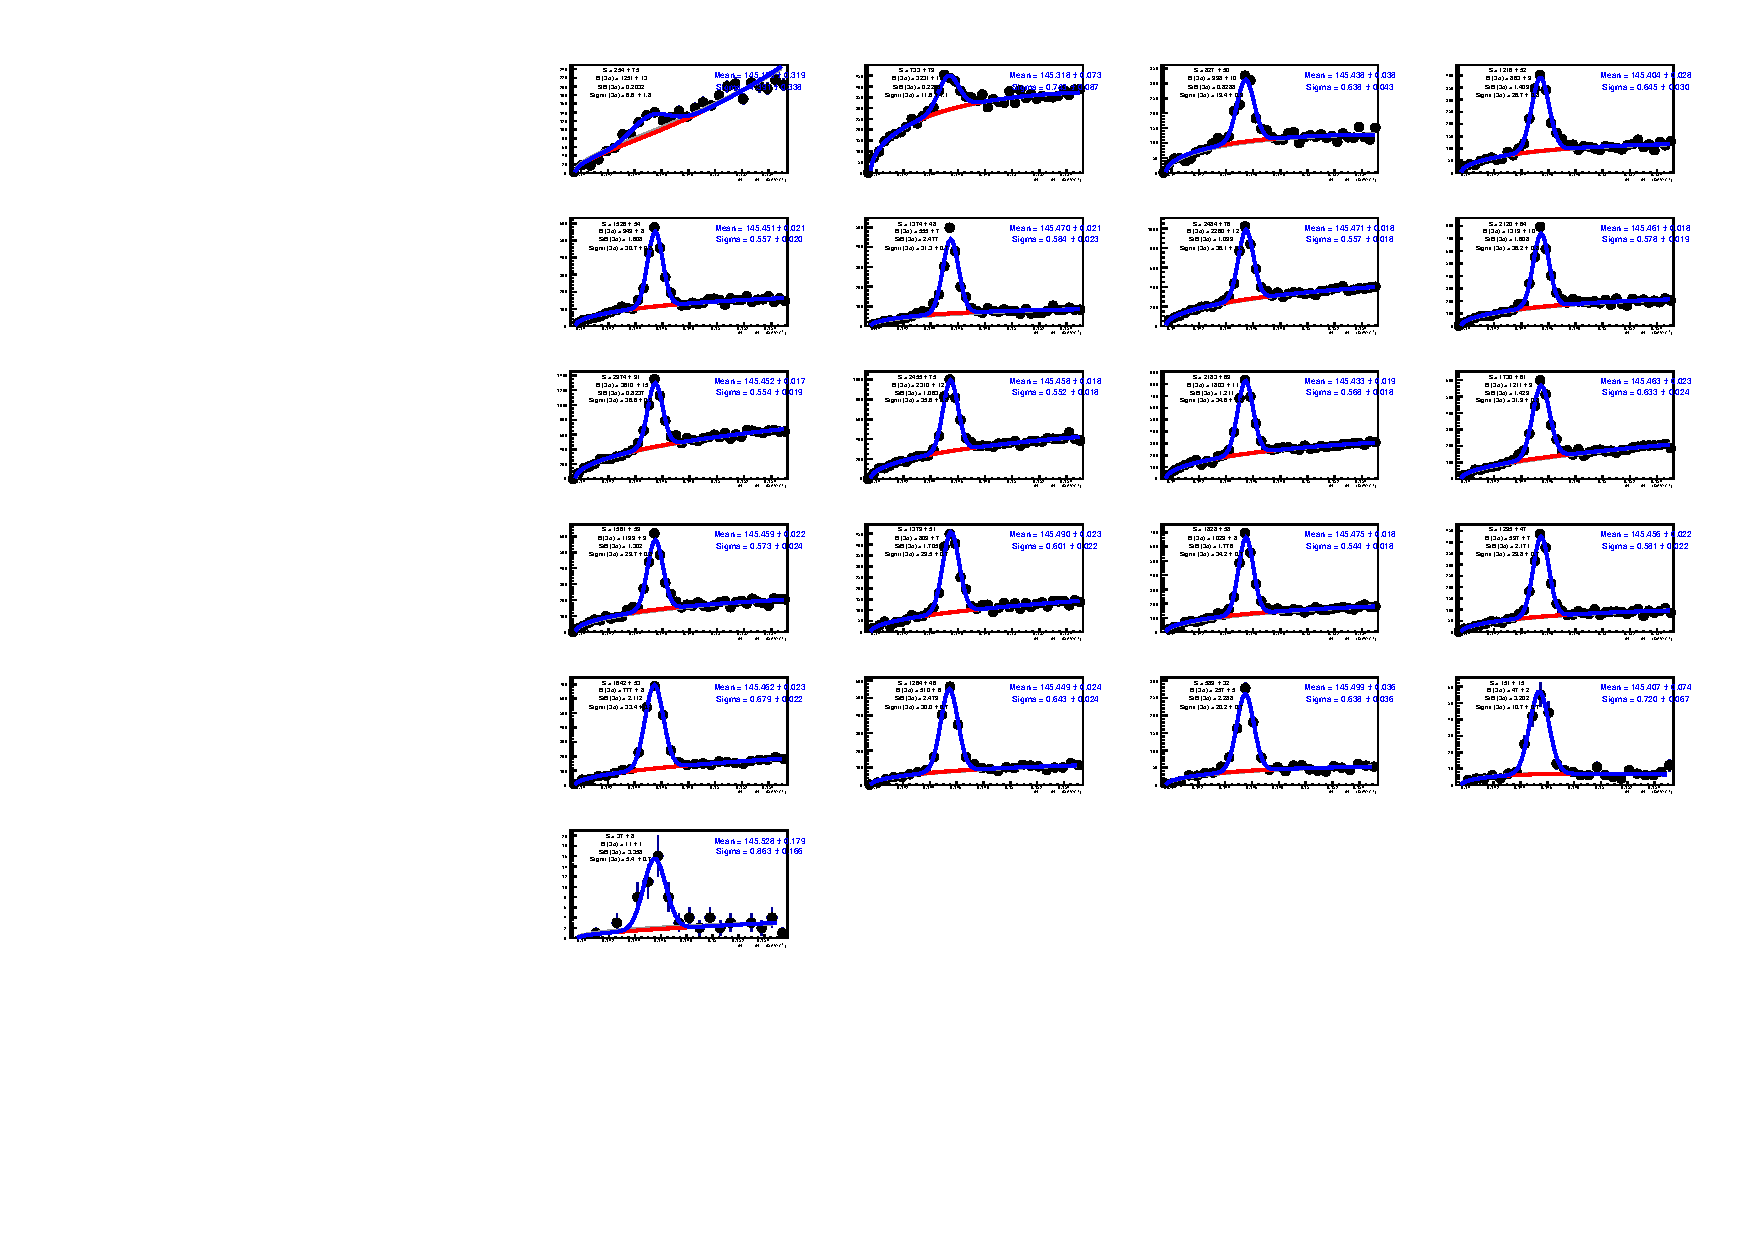
\includegraphics[width=1\textwidth]{figures/Dstar/pp13TeV/DstarInvMass_new.pdf}
\caption{Invariant mass distributions of  (\Dstar -- \Dzero) candidates and charge conjugates in the range 1$<$ \pt$<$ 50 GeV/$c$.}
\label{fig:Dstar_InvMass}
\end{center}
\end{figure}


Similarly the signal for all the four mesons was extracted in the 30--50$\%$ centrality class in several transverse momentum regions: 
\begin{itemize}
	%\item for \Dzero in the range 1-50 GeV/$c$;
	\item for \Dstar in the range 2-36 GeV/$c$;
	%\item for \Dplus in the range 2-50 GeV/$c$;
	%\item for \Dsubs in the range 3-24 GeV/$c$;
\end{itemize} 

The invariant mass distributions obtained in 30--50$\%$ centrality class are reported in Fig.~\ref{fig:Dstar_InvMass2} for \Dstar.


% Dstar 30-50%


The goodness of the mass fit against the Monte
Carlo expectations was checked in terms of mass peak $\sigma$ and position.
The comparisons of the Gaussian width and mean of the \Dstar meson mass peaks in data and Monte Carlo are reported in ~\ref{fig:Dstar_Mean_width}.

% Dstar Mean and width Data vs MC 0-10%


% Dstar Mean and width Data vs MC 30-50%
\begin{figure}[tb]
\begin{center}
 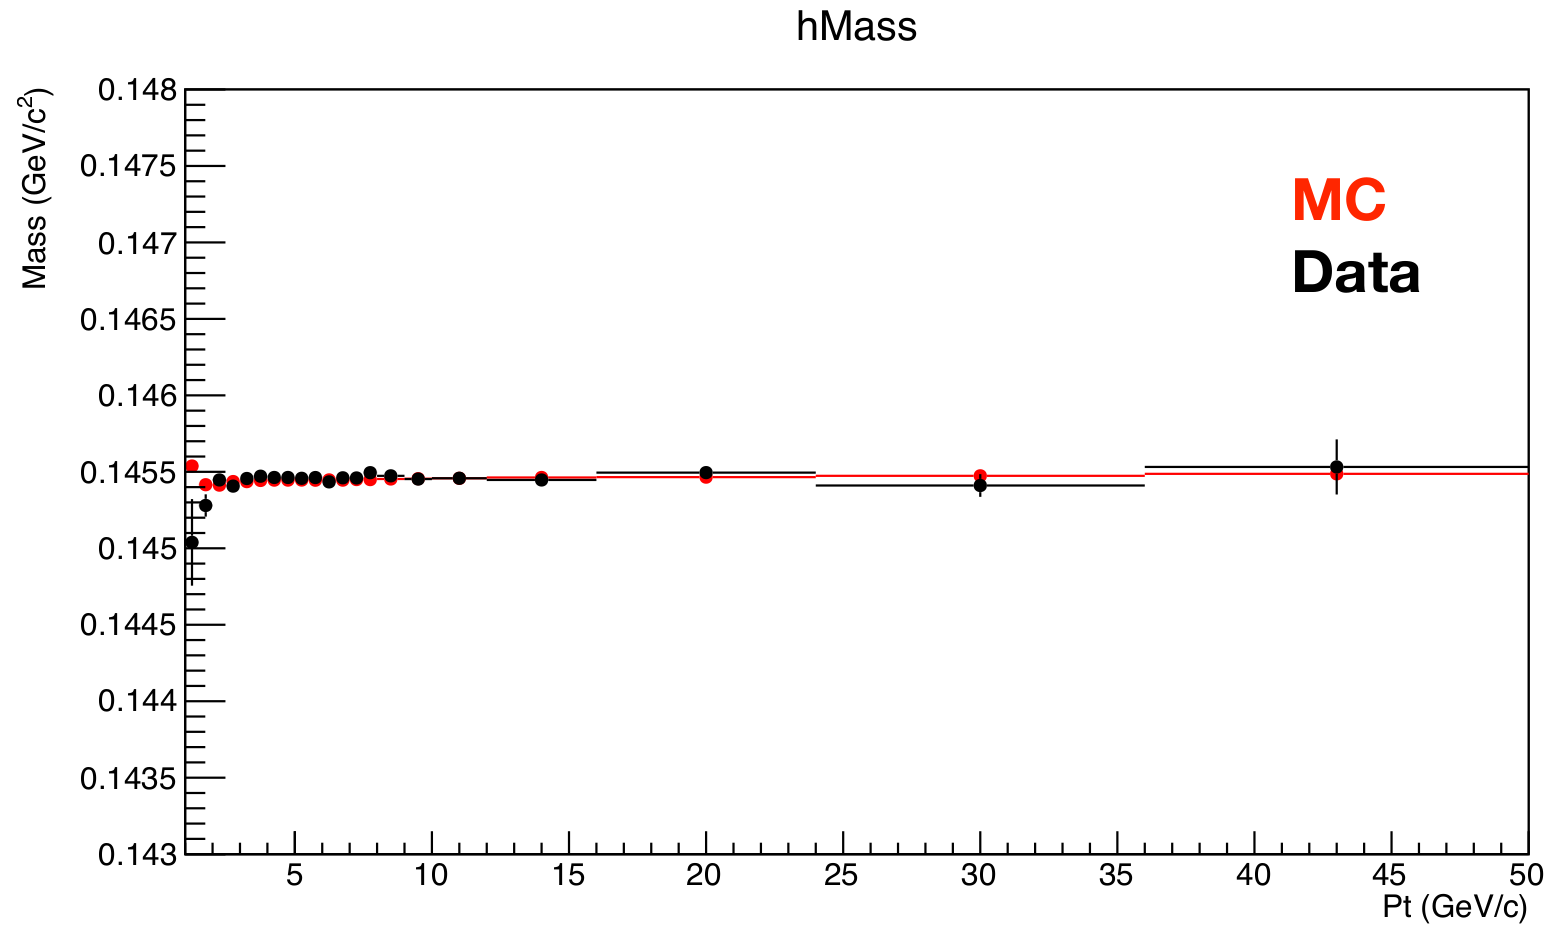
\includegraphics[width=0.65\textwidth]{figures/Dstar/pp13TeV/DstarMean-position.png}
 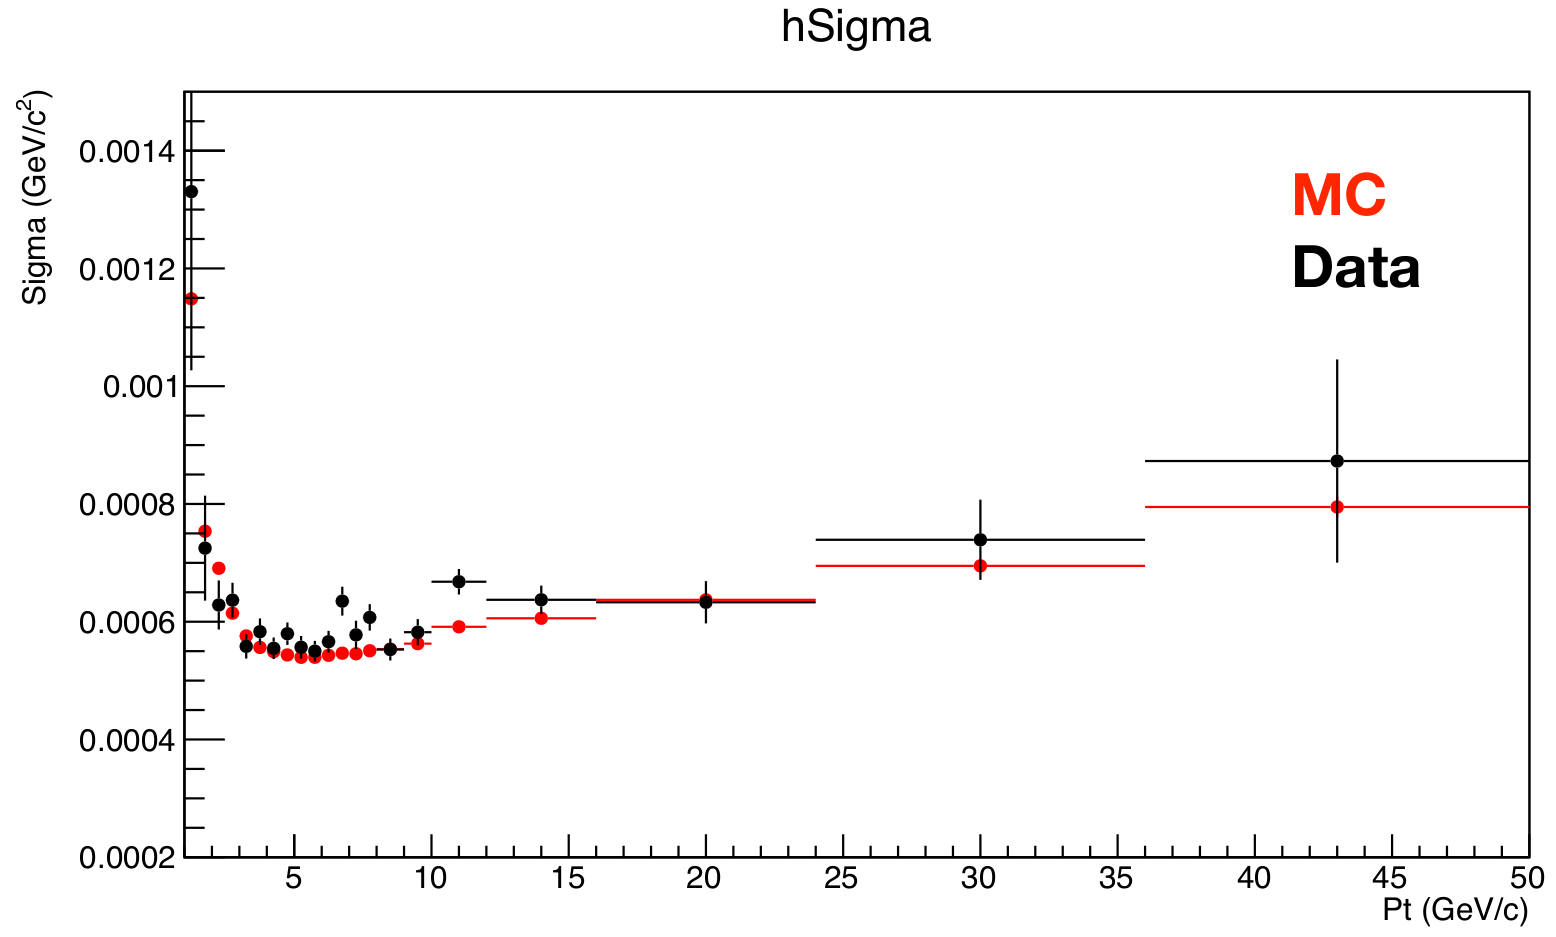
\includegraphics[width=0.65\textwidth]{figures/Dstar/pp13TeV/DstarWidth_sigma.png}
\caption{Comparison of Gaussian mean (left) and width (right) extracted from the invariant-mass fits of \Dstar candidates (black) and the MC simulation (red).}
\label{fig:Dstar_Mean_width}
\end{center}
\end{figure}


% Dplus 0-10% Mean and Width
%\begin{figure}[tb]
%\begin{center}
% \includegraphics[width=1\textwidth]{figures/Dplus/010/meansigma_Comp_010_Pol2andExpo.pdf}
% \caption{Comparison of Gaussian mean (left) and width (right) extracted from the invariant-mass fits of \Dplus candidates in 0--10\% for the data and the MC simulation.}
%\label{fig:Dplus_Mean_width}
%\end{center}
%\end{figure}

% Dplus 30-50% Mean and Width
%\begin{figure}[tb]
%\begin{center}
% \includegraphics[width=1\textwidth]{figures/Dplus/3050/meansigma_Comp_3050_Pol2andExpo.pdf}
% \caption{Comparison of Gaussian mean (left) and width (right) extracted from the invariant-mass fits of \Dplus candidates in 30--50\% for the data and the MC simulation.}
%\label{fig:Dplus_Mean_width2}
%\end{center}
%\end{figure}




% Dstar 30-50%




%\begin{figure}[tb]
%\begin{center}
% \includegraphics[width=0.48\textwidth]{figures/Dsubs/010/Mean_Data_MC.pdf}
% \includegraphics[width=0.48\textwidth]{figures/Dsubs/010/Sigma_Data_MC.pdf}
%\caption{Comparison of Gaussian mean (left) and width (right) extracted from the invariant-mass fits of \Dsubs candidates in 0--10\% for the data and the MC simulation.}
%\label{fig:DsubsMCcomp_cent}
%\end{center}
%\end{figure}

%\begin{figure}[tb]
%	\begin{center}
%	 \includegraphics[width=0.48\textwidth]{figures/Dsubs/3050/CompMean.pdf}
%	 \includegraphics[width=0.48\textwidth]{figures/Dsubs/3050/CompWidth.pdf}
%	\caption{Comparison of Gaussian mean (left) and width (right) extracted from the invariant-mass fits of \Dsubs candidates in 30--50\% for the data and the MC simulation.}
%	\label{fig:DsubsMCcomp_semicent}
%	\end{center}
%	\end{figure}
